\documentclass{article}
\usepackage[margin=1in]{geometry}
\usepackage{graphicx}
\usepackage[outdir=./]{epstopdf}  					% Avoids errors when input figures
\usepackage[labelsep=period,labelfont=bf]{caption}
\usepackage{subcaption}
\usepackage{pdflscape}
\usepackage{afterpage}
\input{../../../Settings/macros_global}			   % Personalized commands
\input{../../../Settings/macros_local}			    % Personalized commands
%\pagestyle{empty}

\begin{document}
	\afterpage{
	\begin{landscape}
	\begin{figure}[tbph]
		\caption{Response of the Yield Curve to Target and Path Surprises} \label{fig:LPYC}
		\begin{center}
			\begin{minipage}{\linewidth}
				\begin{center}
					\begin{subfigure}[t]{\linewidth}
						\includegraphics[trim={0.3cm 0.23cm 0.3cm 0.23cm},clip,height=0.33\textheight,width=\linewidth]{../Figures/LPs/Target/Target11YC.eps} \\
%						\includegraphics[trim={0.3cm 0.23cm 0.3cm 0.23cm},clip,height=0.33\textheight,width=\linewidth]{../Target/Target11YC} \\
						\vspace{-0.35cm}
						\caption{Target Surprises} \label{subfig:Target11YC}
						\vspace{0.4cm}
					\end{subfigure}
				
					\vspace{0.1cm}
					
					\begin{subfigure}[t]{\linewidth}
						\includegraphics[trim={0.3cm 0.23cm 0.3cm 0.23cm},clip,height=0.33\textheight,width=\linewidth]{../Figures/LPs/Path/Path11YC.eps} \\
%						\includegraphics[trim={0.3cm 0.23cm 0.3cm 0.23cm},clip,height=0.33\textheight,width=\linewidth]{../Path/Path11YC} \\
						\vspace{-0.35cm}
						\caption{Path Surprises} \label{subfig:Path11YC}
					\end{subfigure}
					\vspace{-0.45cm}
				\end{center}
				\fignotes{This figure plots the coefficient estimates and 95\% confidence intervals for 1 basis point target and path tightening surprises for yield changes from close of day \(t - 1\) to day \(t + \idxh\), where \(t\) is a day with a monetary policy announcement and \(\idxh = 0, 1, \ldots, 30\). An arrow in the vertical axis indicates the contemporaneous effect (when \(\idxh = 0\)). The surprises are equal to the target and path surprises (obtained with intraday data) on announcement days and zero otherwise. The sample includes all regular monetary policy announcements from January 2011 to \lastobs. The 95\% confidence bands are based on robust standard errors.}
			\end{minipage}
		\end{center}
	\end{figure}
	\end{landscape}
	}
\end{document}
% trim = {<left> <lower> <right> <upper>}